%
% Another appendix chapter
\chapter{Application: Walking}\label{chap:walking}
The control strategy for a static, standing case presented in the previous chapter is two-dimensional. If the robot is walking, the horizontal \ac{CoM} position can lie outside the support polygon. The result of this is that the desired \ac{CoP} cannot always be placed in line with the \ac{ICP} error.  In this chapter, the bang-bang control law of Chapter \ref{chap:standing} is extended for the use while the robot is walking.
% Experimental Setup
\section{Experimental Setup}
In this section, to determine \textit{when} to turn the bang-bang controller on in \ac{3D},  tests are conducted preliminary to developing a controller. In the tests, a push is applied in the beginning of the \ac{SS} while the robot is walking. The stepping parameters used for the test situation are given in Table \ref{tab:stepping}, which are the default stepping parameters during testing in simulation. In \figref{fig:valwalkingtest}, the test setup in simulation is shown. The limited foothold options display that footstep location adjustment is not available as a balance strategy. In \figref{fig:3foot}, the \ac{ICP} and \ac{CMP} reference trajectory and the measured \ac{CoM} trajectory, without application of a push are made visible. 
\begin{table}
\caption{Stepping Parameters} % title of Table
\centering % used for centering table
\begin{tabular}{c c c } % centered columns (4 columns)
\hline\hline %inserts double horizontal lines
Parameter & Value & Unit \\
%heading
\hline % inserts single horizontal line
Step Legth & 0.5 &  [m]\\
Step Width & 0.25 & [m]\\
\acs{SS} Time & 0.6 & [s]\\
\acs{DS} Time & 0.15 & [s]\\
%[1ex] % [1ex] adds vertical space
\hline %inserts single line
\end{tabular}
\label{tab:stepping} % is used to refer this table in the text
\end{table}
\begin{figure}[h]
\centering
  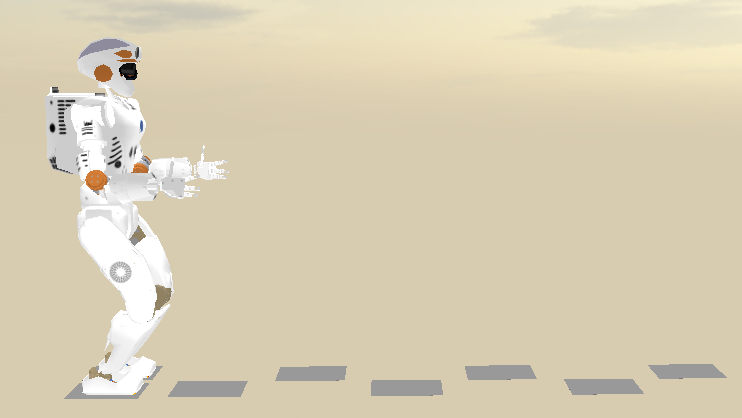
\includegraphics[width=.8\linewidth]{STYLESTUFF/valwalkingtest.png}
   \caption{Test setup for push recovery during walking in simulation. The limited foothold options show that footstep adjustment is not available as a balance strategy.}
    \label{fig:valwalkingtest}
\end{figure}
\begin{figure}[h]
\centering
  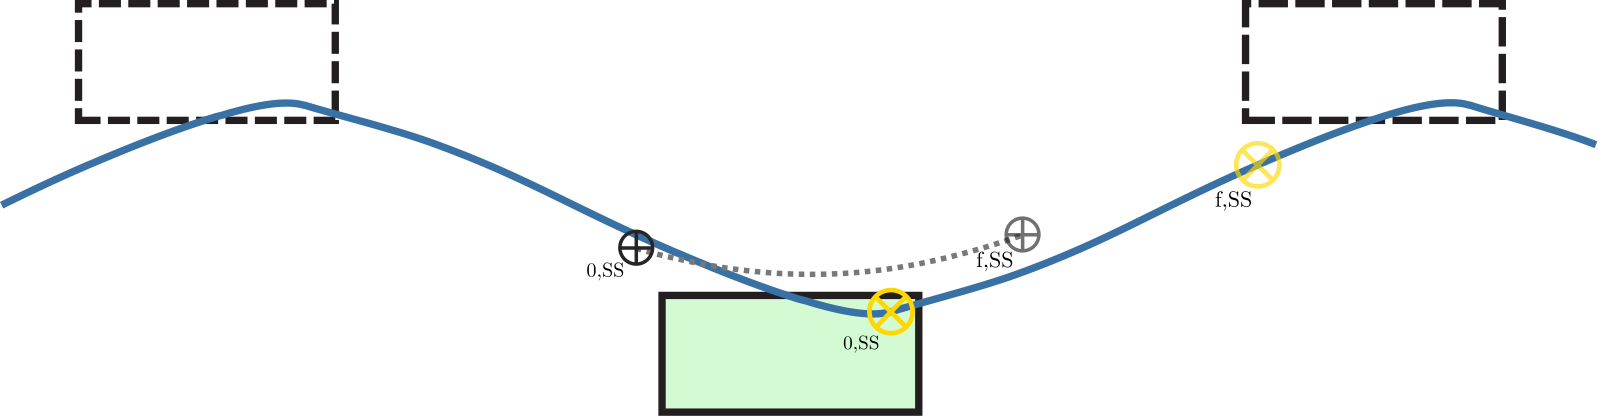
\includegraphics[width=.8\linewidth]{STYLESTUFF/ICPplan3StepComICPrSS.png}
   \caption{Trajectories during \ac{SS} in the horizontal plane (gray dotted lines). The gray area is the current footstep position.}
    \label{fig:3foot}
\end{figure}
%Preliminary observations

The following properties are observed, when applying pushes in different direction in the start of \ac{SS}:
\begin{enumerate}
	\item The direction of the \ac{ICP} error stays often approximately the same until transition to \ac{DS}.
	\item If the \ac{ICP} error is directed in the sagittal plane, the desired \ac{CMP} often remains somewhat in the same location.
	\item If the \ac{ICP} error is directed  in the coronal plane, the desired \ac{CMP} slides from back to the forth of the foot.
	\item The configuration and velocity near transition to \ac{DS} affects the robots ability to put its swing leg down at the desired time. 
\end{enumerate}
These properties are used as assumptions in the development of a control law.
% Methods
\section{Method}
The control law of the previous chapter is first adjusted for desired \ac{CMP} positions outside the support polygon. Second, control variables are introduced, which are used to select one of three predefined control actions.

\subsection{Avoiding Generating Additional Angular Momentum Rate}
First, the control law of the previous chapter is made suitable for $\rcmpd$ locations outside the support polygon. The motivation in the development of a control law is to request as less as possible additional angular momentum rate compared to the default setup, when using \ac{CoM} height variations for balance control. Therefore, the vertical motion controller generates an added desired momentum rate on top of the default controller if $\rcmpd$ is outside the support polygon. Under the assumption that the difference in $\rcopd$ and $\rcmpd$ is directly related to the resulting torque about the \ac{CoM}, the following is derived:
\begin{align}
    \dotldxy &= \frac{\cxy-\rcmpd}{z}(mg+\dotldz),\\
&=\frac{\mathbf{c}_{xy}-\Big(\rcopd+\frac{\taucom}{(mg+\dotldz)}\Big)}{z}(mg+\dotldz), \\
&=\frac{\mathbf{c}_{xy}-\rcopd}{z}(mg + \dotldz)- \frac{\taucom}{z},
\end{align}
If the location of $\rcmpd$ is outside the polygon, the vertical motion controller uses $\rcopd$ for additional height variation. The computation reads as follows:
 \begin{align}
\dot{\mathbf{l}}_{xy,d}&=\frac{\mathbf{c}_{xy}-\rcopd}{z}(mg+\dotldz) - \frac{\taucom}{z},\\
&\approx \underbrace{ \frac{\mathbf{c}_{xy}-\mathbf{r}_{cmp,d}} {z_0}mg}_{\dotldxylip}  + \underbrace{\frac{\mathbf{c}_{xy}-\mathbf{r}_{cop,d}}{z}\dotldz}_{\dotldxyheight},
\end{align}
where $\dotldxyheight$ is the additional desired horizontal linear momentum rate from the vertical motion controller and $\dotldxylip$ the momentum rate from the default control law.

In Figure \ref{fig:rcopdvsrcmpd}, it is visually explained how this computation of $\dotldxy$ does not require additional angular momentum rate from the robot. However, the resulting \ac{CMP} location would be different.

\begin{figure}
\centering
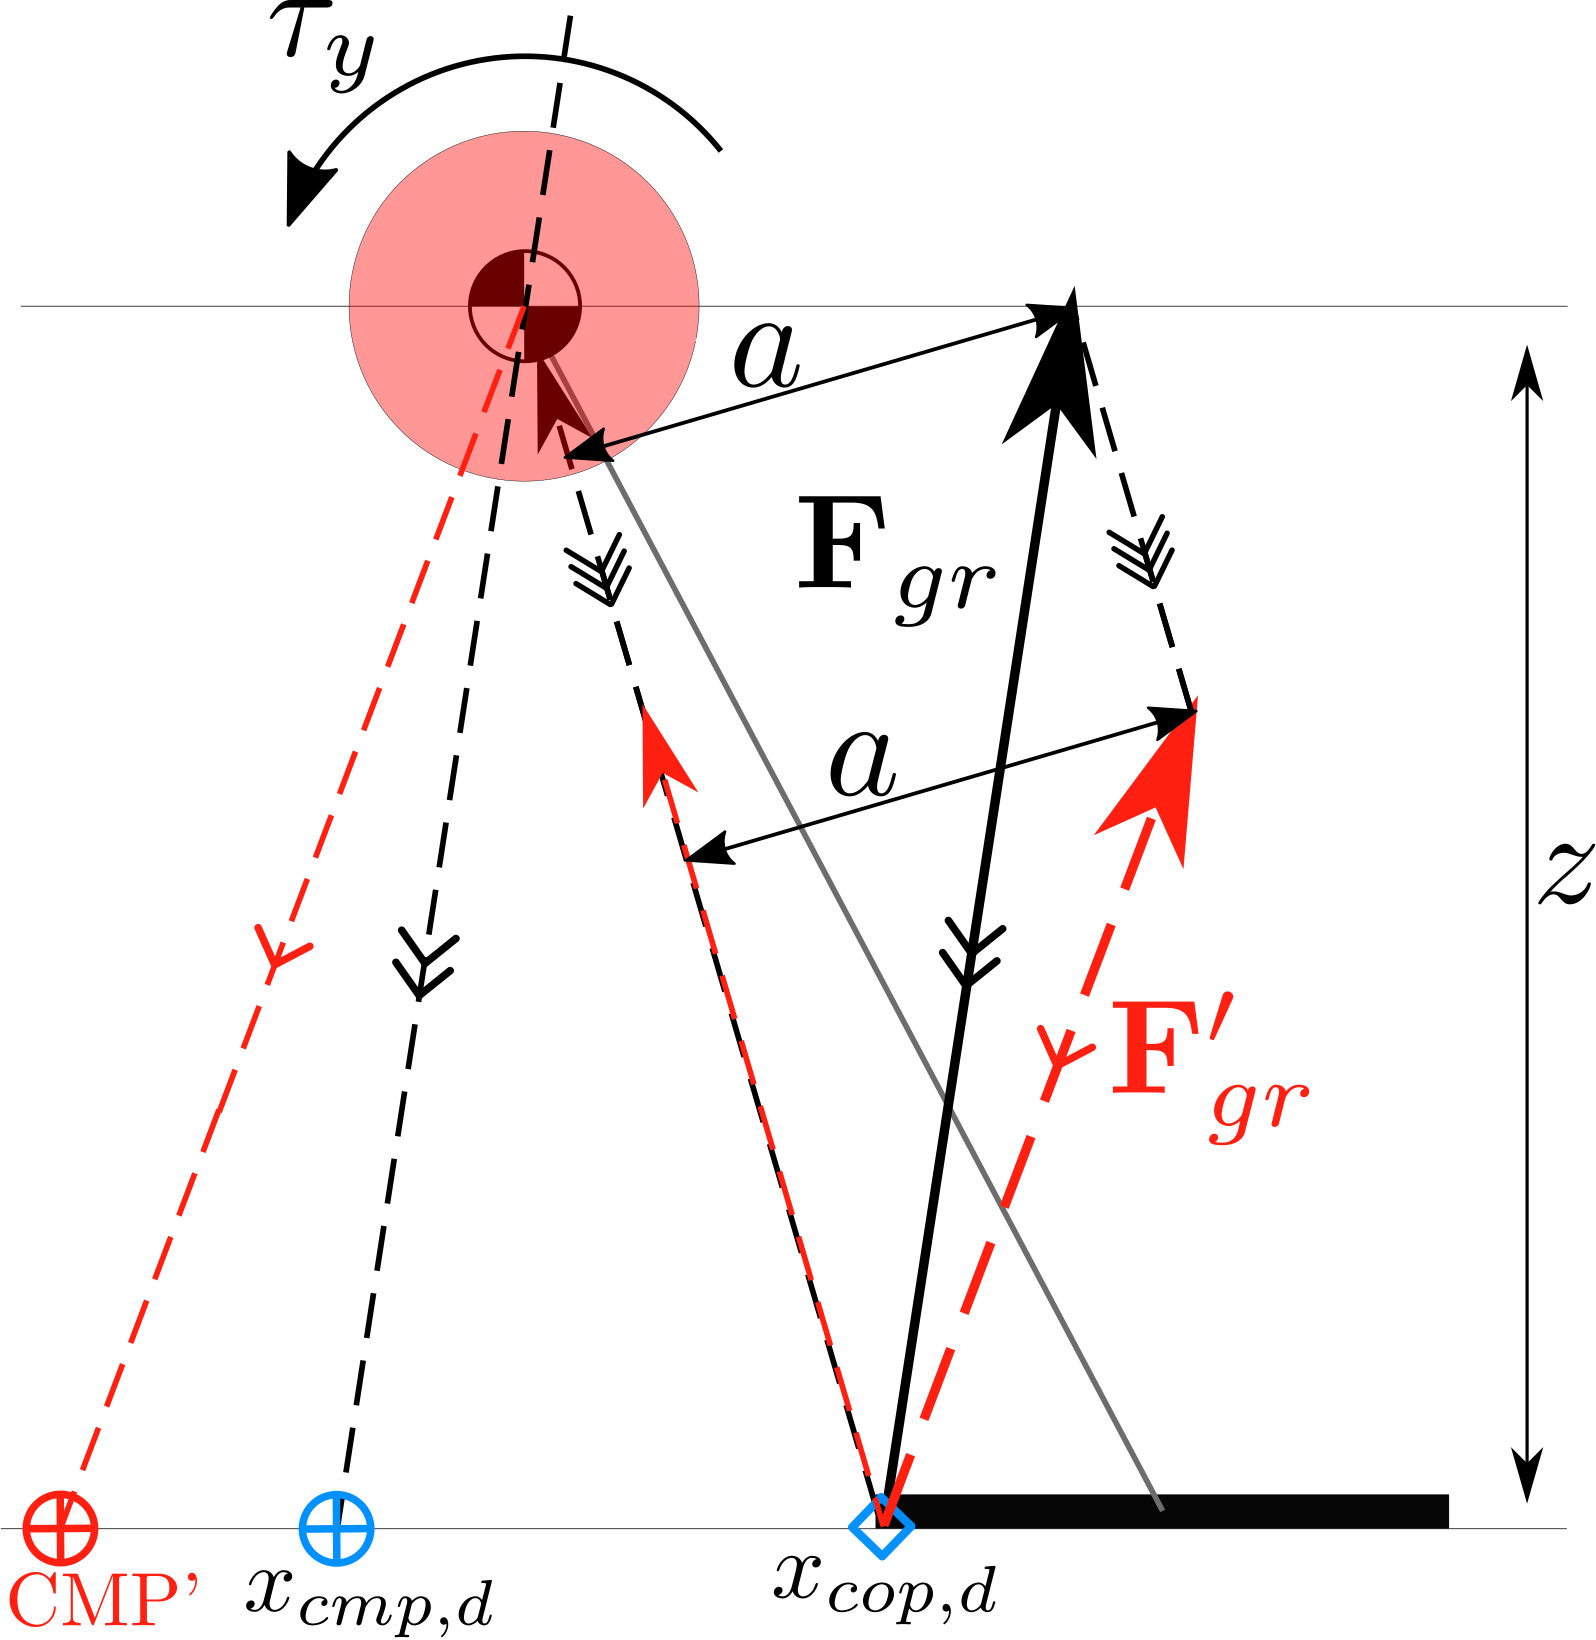
\includegraphics[width=0.45\textwidth]{STYLESTUFF/2DControlStrategyViz.png}
\caption{Requesting additional horizontal momentum rate based on $\rcopd$ will not need additional angular momentum to be achievable, as the scalar offset $a$ is equal. However, the resulting \ac{CMP} will be in a different location than $\rcmpd$.}
\label{fig:rcopdvsrcmpd}
\end{figure}
\subsection{Alignment Angle and Relative Distance}
If the \ac{CoM} is outside the support polygon, the local virtual leg between $\rcopd$ and the horizontal \ac{CoM} location $\cxy$ may not be aligned with direction of the \ac{ICP} error $\icpe$. This results in the leg applying force in a different direction than is needed to cancel the error, which can result in additional error in another direction. Also, if $\cxy$ is close to the polygon edge, the distance with $\rcopd$ might be very small, such that height changes have little to potentially no effect. To take these two aspects into account, the following variables are introduced, which help to determine when to use \ac{CoM} height variation for balance:
\begin{itemize}
	\item $\phi$: the alignment angle between the virtual leg between $\rcopd$ and $\cxy$ and the \ac{ICP} error $\icpe$;
	\item $\delta$: the effective distance between $\rcopd$ and $\cxy$. The is the distance between the two points in the direction of the \ac{ICP} error $\icpe$.
\end{itemize}

In \figref{fig:phiViz}a-b, the two variables are graphically explained using the stance foot position and configuration of \figref{fig:3foot}. $\rcmpd$ is allowed to move a small distance outside the polygon. In \figref{fig:phiVizc}, the angle $\phi$ is zero and $\delta$ is relatively large. This is a relatively suitable error for height control. In \figref{fig:phiVizd}, the angle $\phi$ is $90$ degrees and therefore the distance $\delta$ is zero. In this configuration, \ac{CoM} height variation would not help driving the error back. Furthermore, an additional error would occur orthogonal to the current $\icpe$.
\begin{figure}[h]
\centering
  \begin{subfigure}{0.49\textwidth}
    \centering
  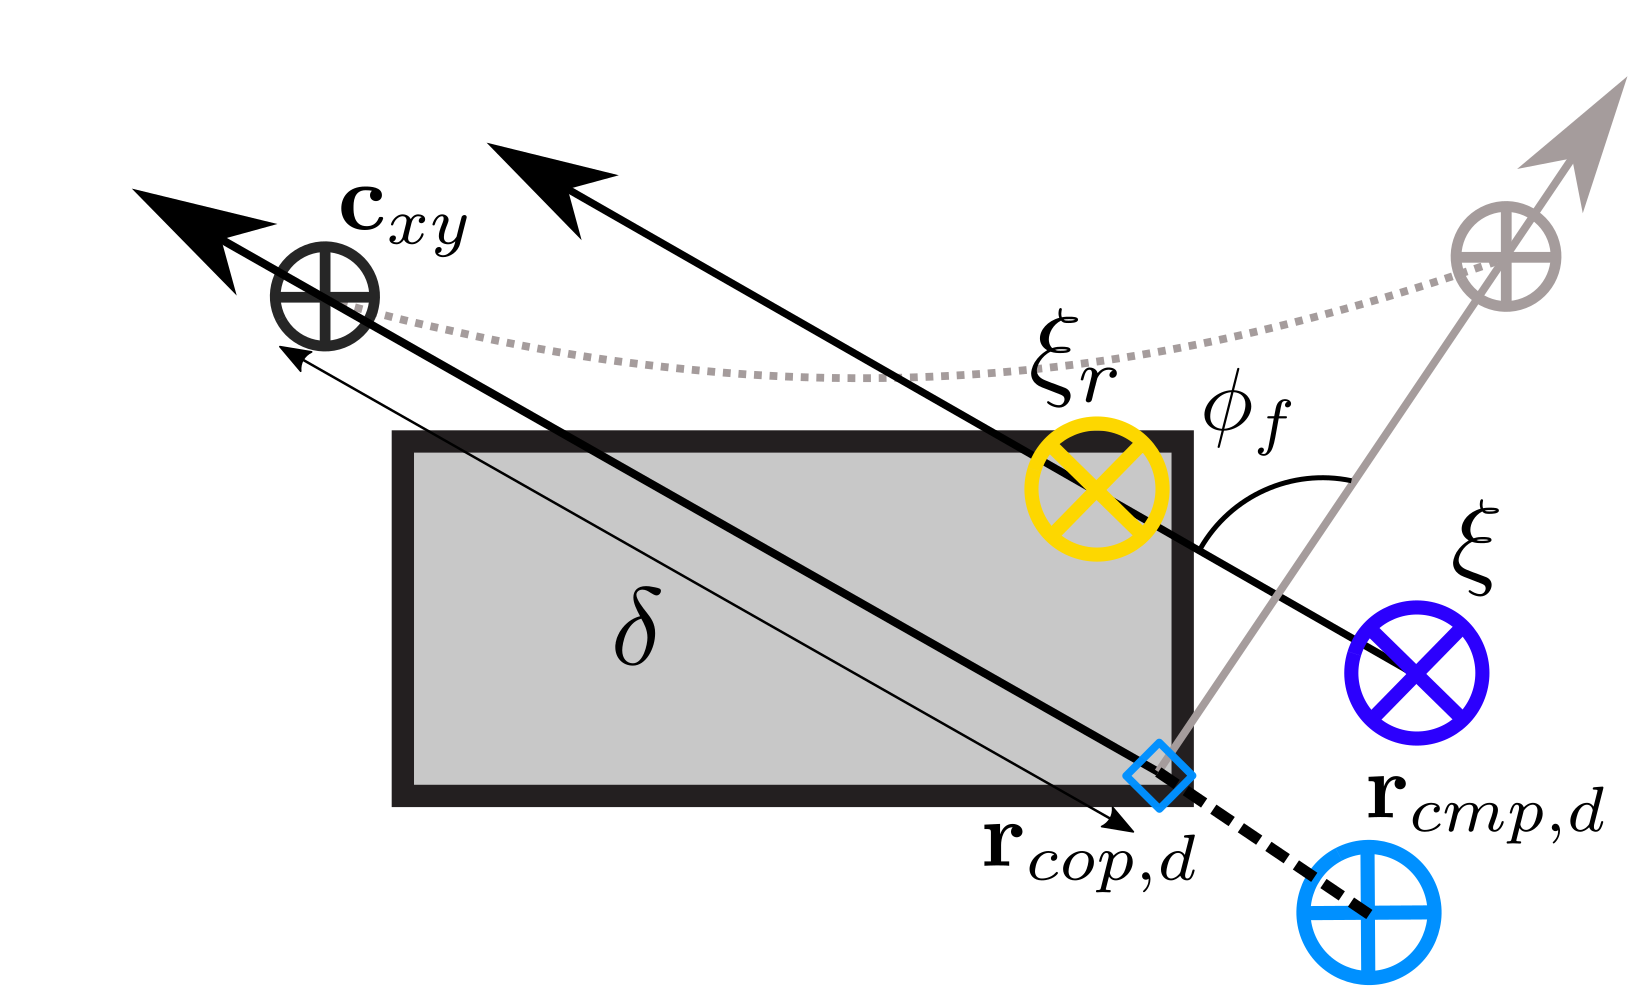
\includegraphics[width=.7\linewidth]{STYLESTUFF/ICPplanStartSSPhiViz0.png}
    \caption{}
     \label{fig:phiVizc}
  \end{subfigure}
  \begin{subfigure}{0.49\textwidth}
    \centering
  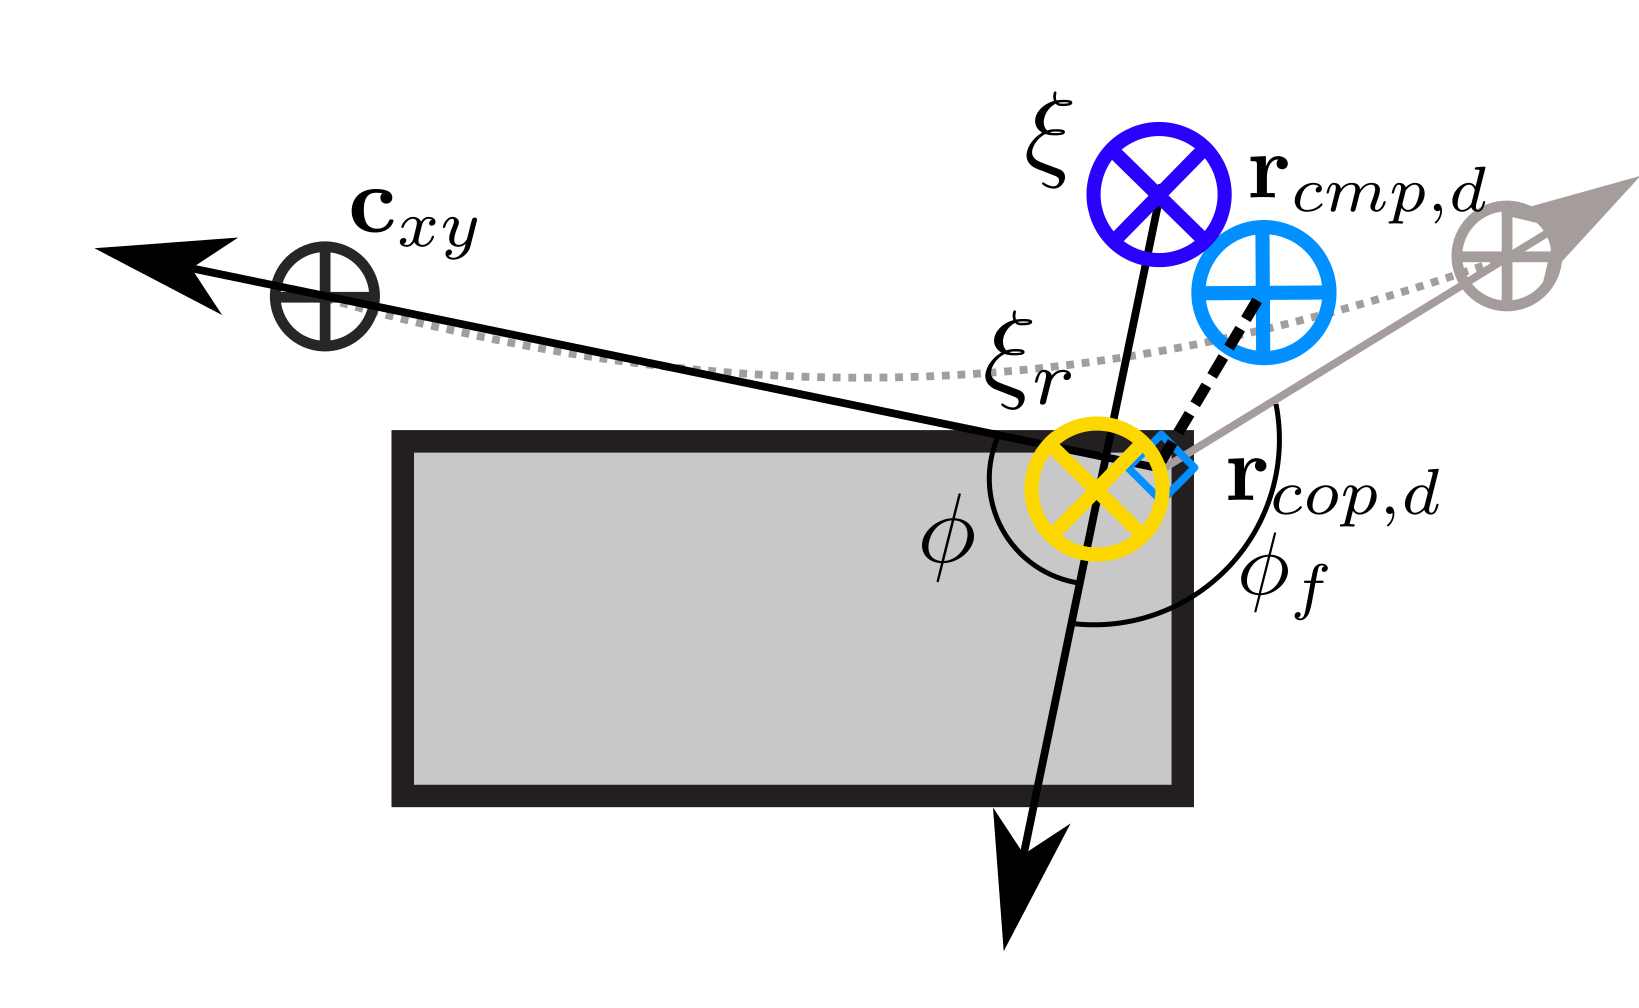
\includegraphics[width=.7\linewidth]{STYLESTUFF/ICPplanStartSSPhiViz90.png}
    \caption{}
     \label{fig:phiVizd}
  \end{subfigure}
  \begin{subfigure}{0.49\textwidth}
  \centering
  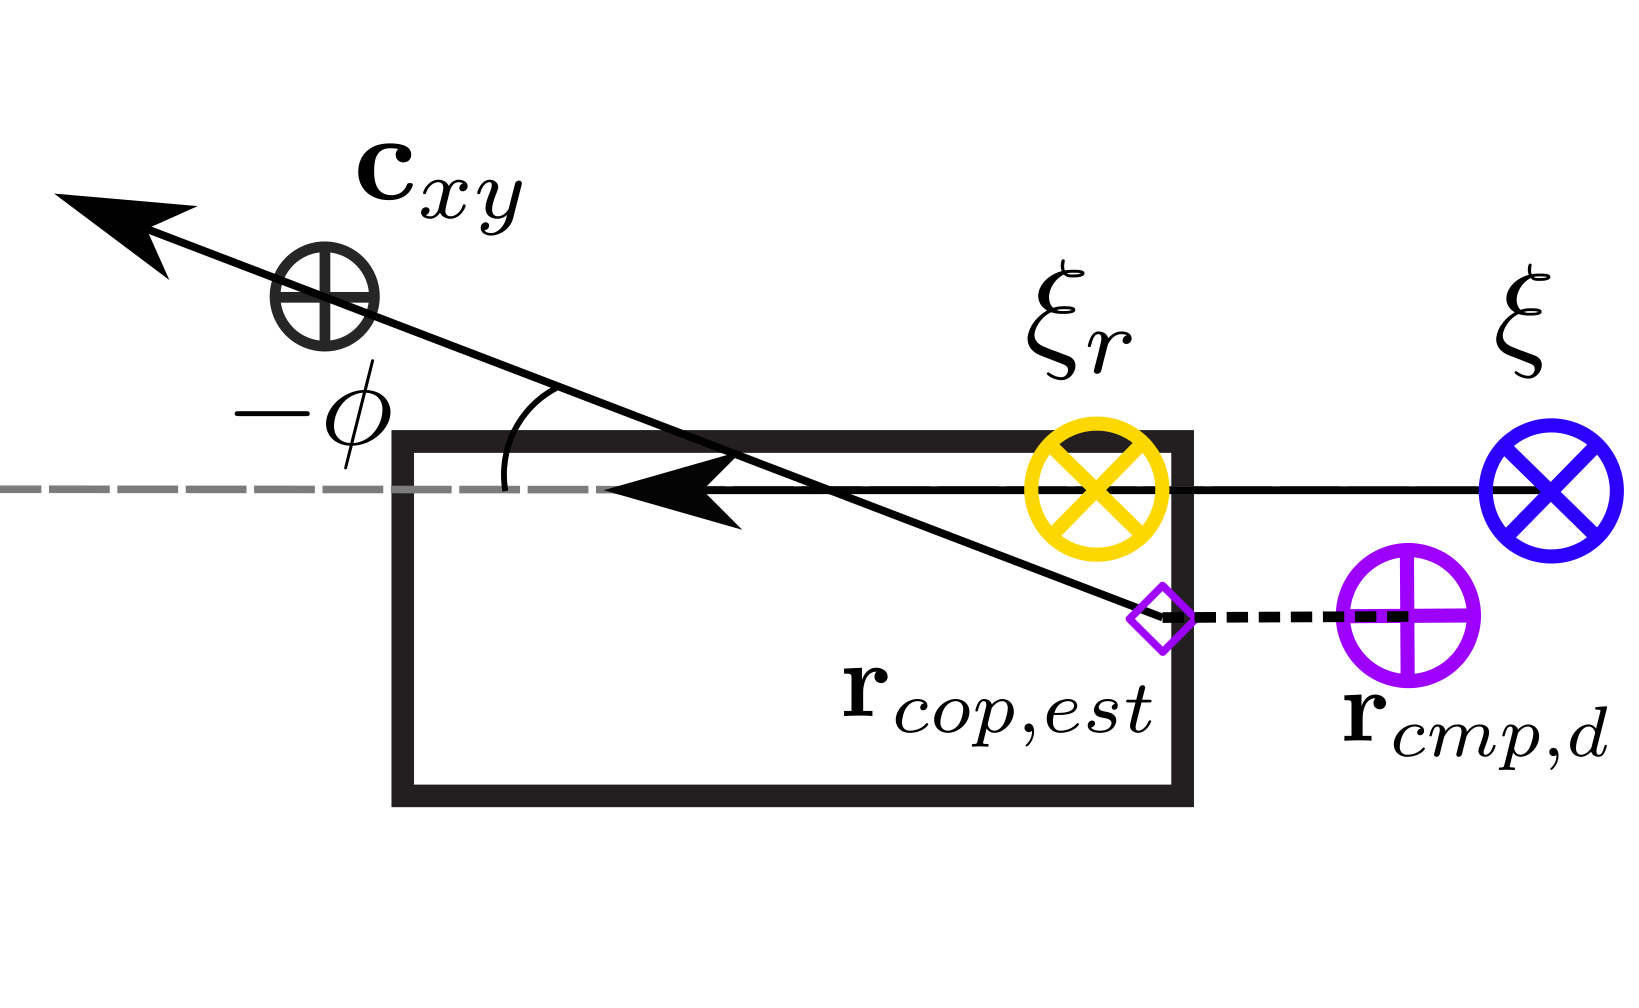
\includegraphics[width=.7\linewidth]{STYLESTUFF/ICPplanStartSSPhiVizNegError.png}
   \caption{}
    \label{fig:phiViza}
  \end{subfigure}
  \begin{subfigure}{0.49\textwidth}
    \centering
  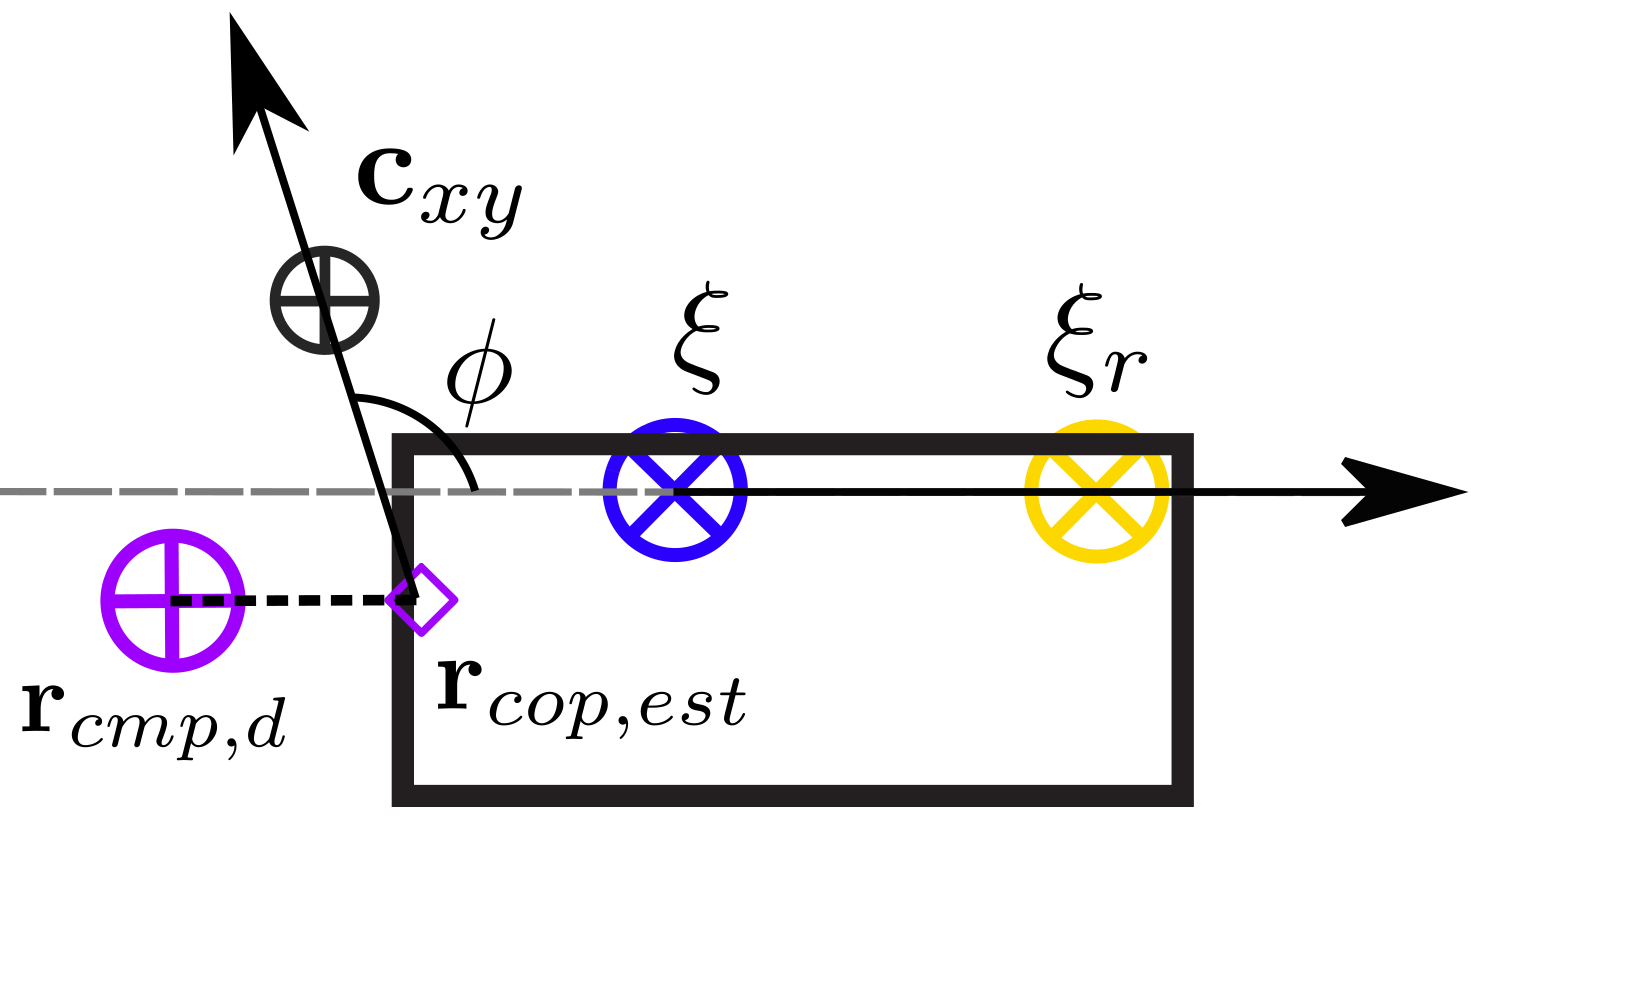
\includegraphics[width=.7\linewidth]{STYLESTUFF/ICPplanStartSSPhiViz.png}
  \caption{}
   \label{fig:phiVizb}
  \end{subfigure}
    \begin{subfigure}{0.49\textwidth}
    \centering
  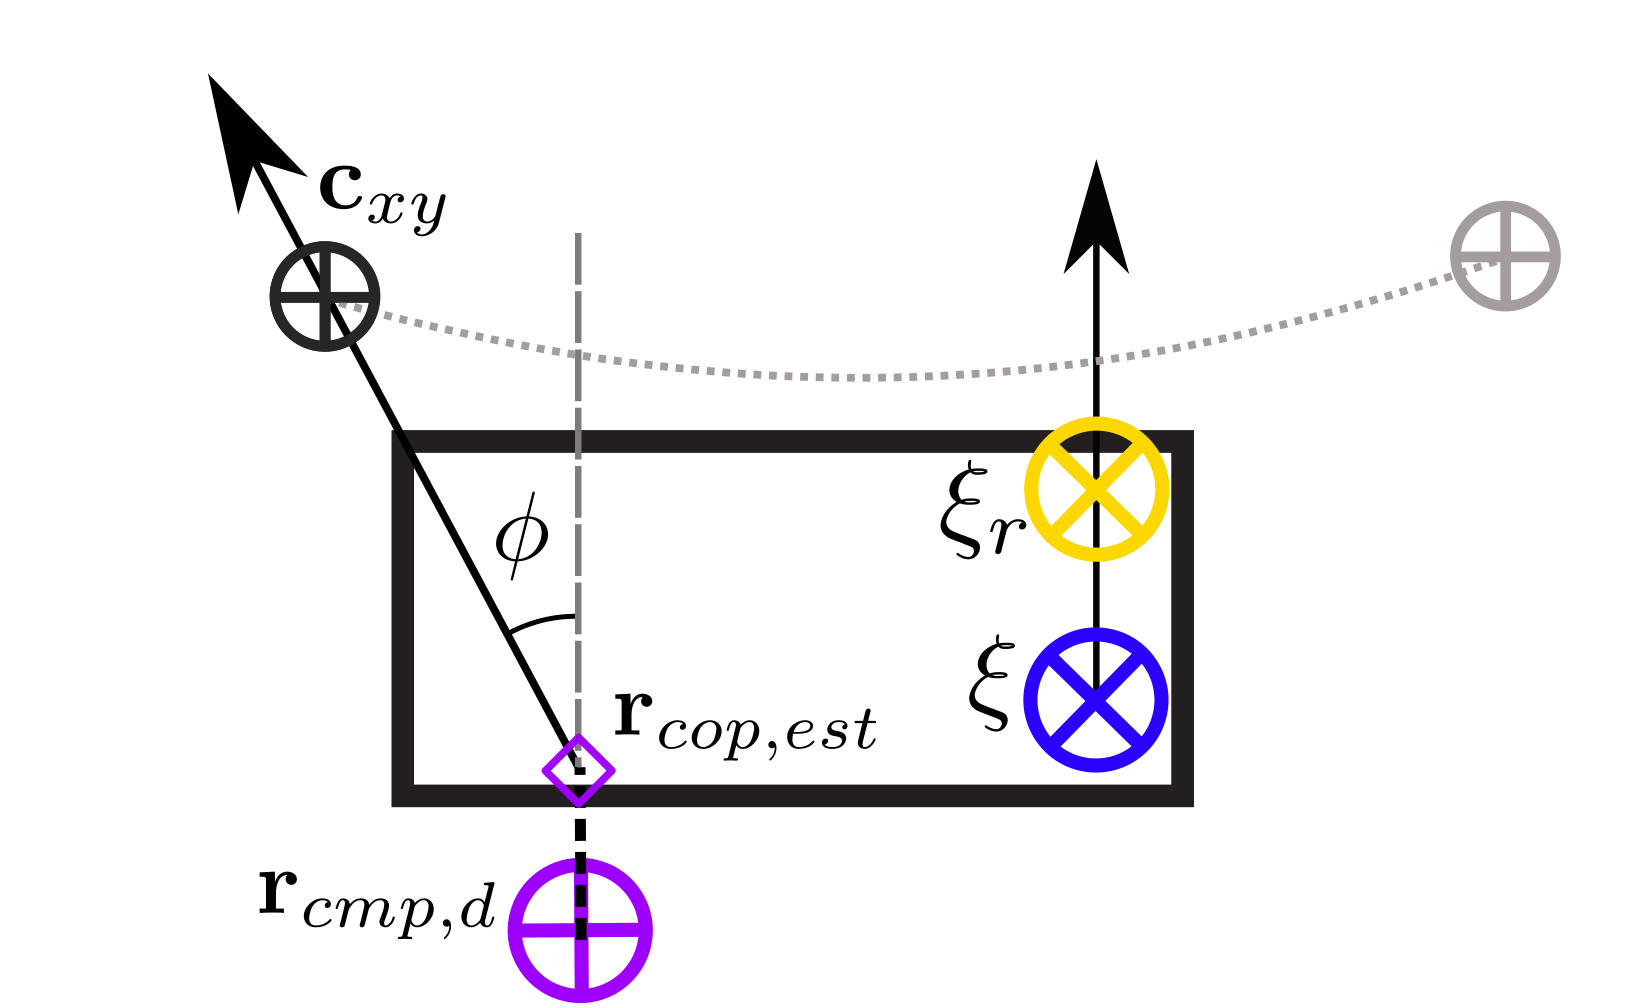
\includegraphics[width=.7\linewidth]{STYLESTUFF/ICPplanStartSSPhiVizLeftError.png}
    \caption{}
     \label{fig:phiVize}
  \end{subfigure}
  \begin{subfigure}{0.49\textwidth}
    \centering
  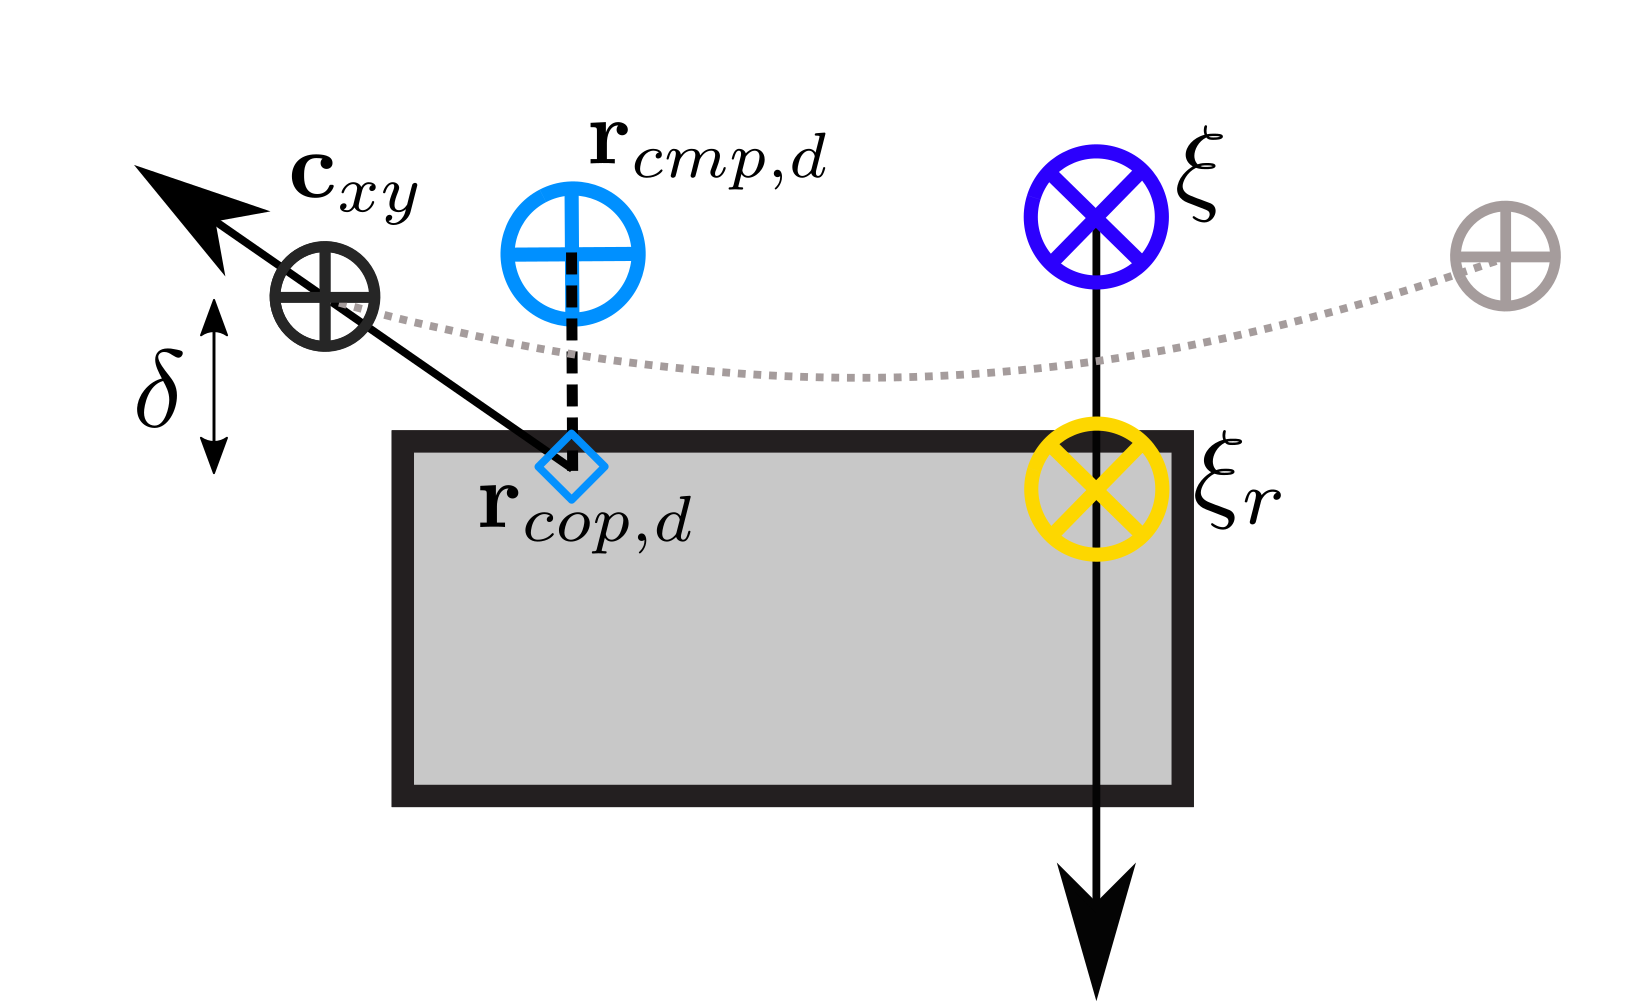
\includegraphics[width=.7\linewidth]{STYLESTUFF/ICPplanStartSSPhiVizRightError.png}
    \caption{}
     \label{fig:phiVizf}
  \end{subfigure}
  \caption{Vizualizations of $\phi$ and $\delta$ for the configuration at start of \ac{SS}.}
  \label{fig:phiViz}
\end{figure}

\subsection{Actions}
The alignment angle $\phi$ and the relative distance $\delta$ are used to select a control action, if $\rcmpd$ crosses the polygon edge. From the assumptions of the preliminary observations $1$ and $2$, it is assumed that the angle $\phi$ will be dependent on the current $\icpe$ and $\rcopd$ throughout \ac{SS} if $\icpe$ is directed in the sagittal plane. Therefore, the additional variables $\delta_f$ and $\phi_f$ are used, which are the expected alignment and distance in the end of \ac{SS}, based on the \ac{CoM} location coming from the \ac{ICP} planner. Also, from assumption $3$, $\phi$ is not used if a push is in the coronal plane. Throughout \ac{SS}, the whole foot length is available for future $\rcmpd$ placements that could correct any additional error. Based on the discussed variables, the following three actions can be selected:
\begin{itemize}
	\item \textbf{Positive alignment}: At the current control tick, $\phi$ is relatively aligned and $\delta$ relatively large for a push in the sagittal plane, or $\delta$ is relatively large for a push in the coronal plane. Also, $\phi$ has to be smaller than $\frac{1}{2}\pi$ [rad], as the virtual leg must be in direction of the \ac{ICP} error to make additional force effective. A bang-bang action is activated that starts with a positive `bang'. The thresholds related to this action are $\phimin < \phi < \phimax$ and $\delta > \deltamin$, where $\phimin$, $\phimax$ and $\deltamin$ are parameters for the minimum and maximum $\phi$ and minimum $\delta$.
	\item \textbf{Prepare}: At the current control tick, $\phi$ is relatively misaligned or $\delta$ is relatively small, but $\phi_f$ and $\delta_f$ are at values suitable for the positive alignment phase. The \ac{CoM} height is gradually lowered to the minimum height, after which the `bang-bang' action of the positive alignment phase is activated. The the thresholds related to this action are $\phimin<\phi_f<\phimax$ and $\delta_f>\deltamin$.
	\item \textbf{Default}: All decisions variables $\phi$, $\delta$, $\phi_f$ and $\delta_f$ are at such values, that vertical \ac{CoM} motion does not improve recovery. The default height control law is used and no additional height changes are considered. The threshold related to this action is if the prepare or the positive alignment thresholds do not hold.
\end{itemize}

In \figref{fig:phiViz}, six cases are shown for different actions. In \figref{fig:phiVizc}, the positive alignment action is used, as the $\delta$ is relatively large and $\phi$ relatively small. In \figref{fig:phiVizd}, the default action is introduced, as $\delta$ is zero and $\phi$ is misaligned. In \figref{fig:phiViza}, the error is a result of a back push. A positive alignment action is introduced, as $\phi$ is relatively small and $\delta$ relatively large. In \figref{fig:phiViza}, a push is applied frontally on the robot. The prepare action is used, as $\delta_f$ and $\phi_f$ are more suitable for height control. In \figref{fig:phiVize}, the robot is pushed from the left. The positive alignment action is used, as the current $\delta$ is relatively large. In \figref{fig:phiVizf}, the error is a result from a push from the right. The default action is activated, as $\delta$ is small throughout \ac{SS}.

For the maximum height constraint $\zmax$, the same parameters as for the standing tests is used in the first half of \ac{SS}. In the second half, the maximum height constraint is linearly interpolated between the maximum height constraint for standing and a maximum height constraint at the end of \ac{SS}.  For the minimum height constraint $\zmin$, a constant value is considered. The height constraints are visually explained in \figref{fig:heightconstraints}.
\begin{figure}
\centering
  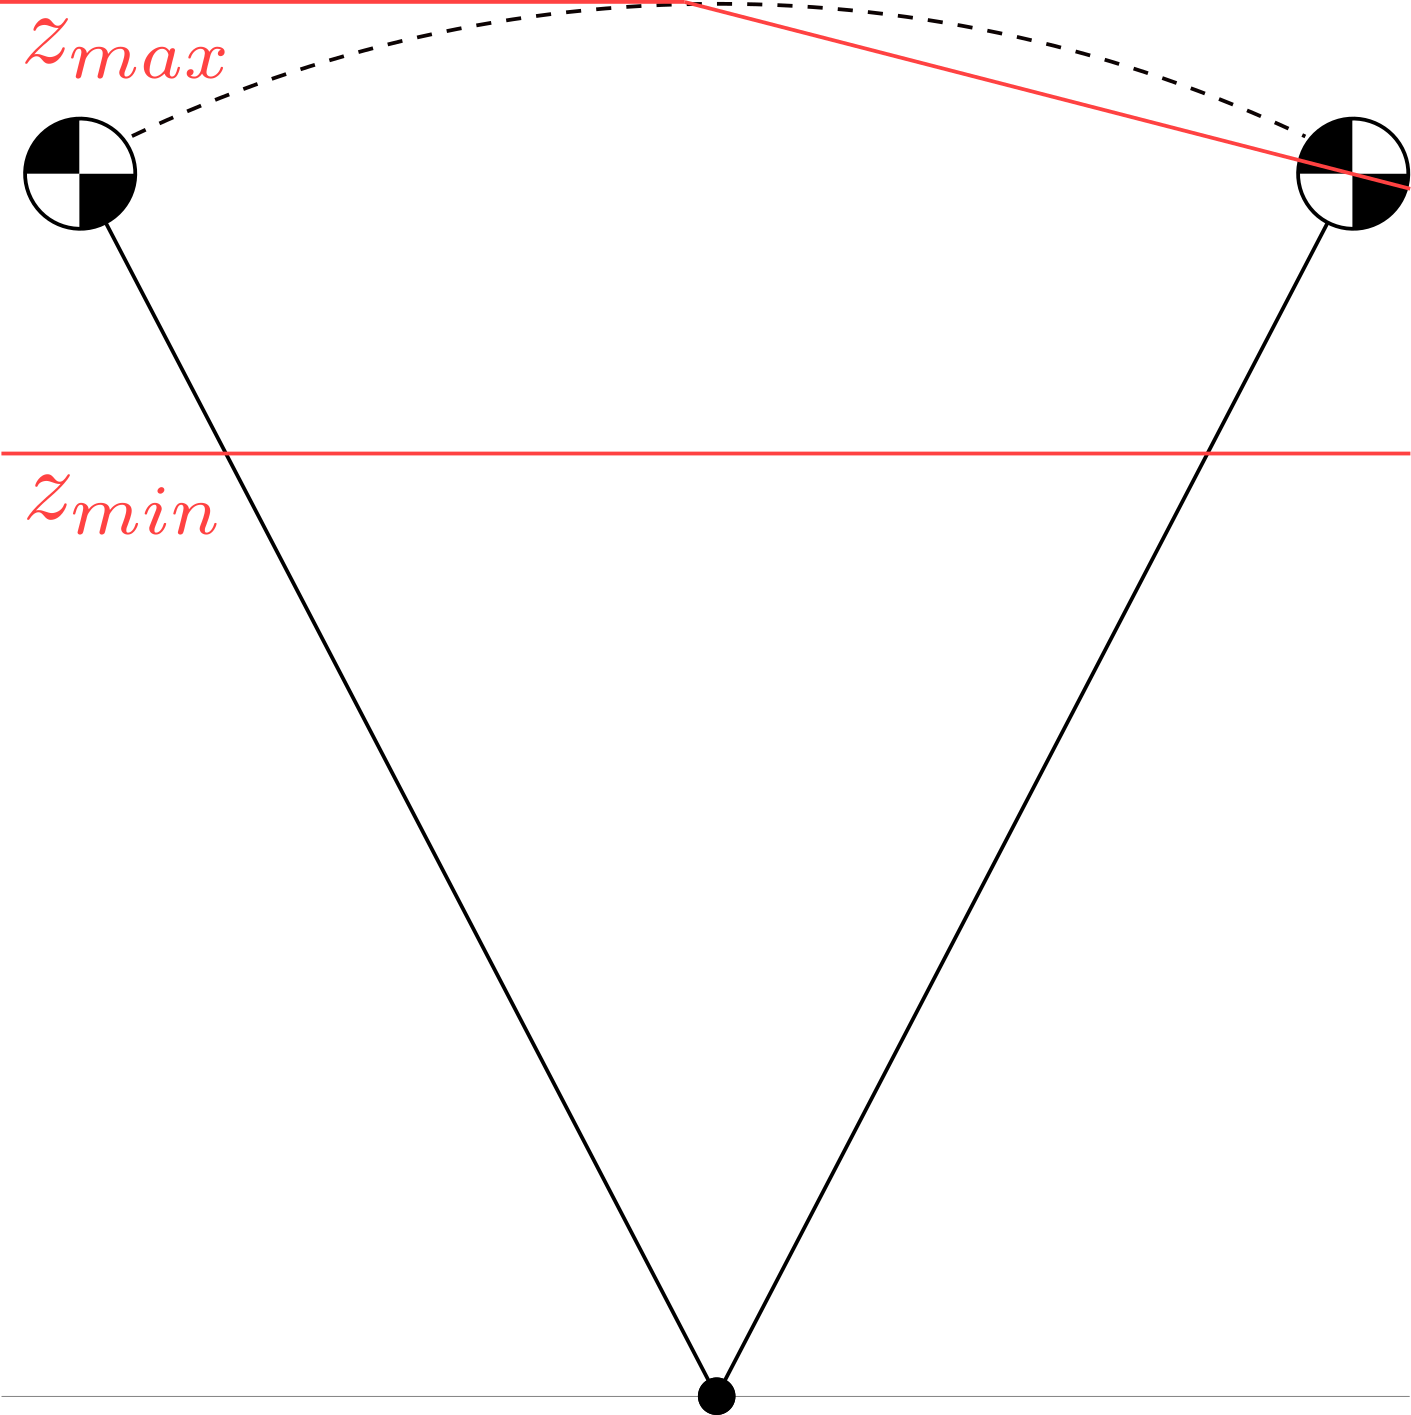
\includegraphics[width=.4\linewidth]{STYLESTUFF/heightconstraints.png}
   \caption{Height constraints through \acf{SS}}
    \label{fig:heightconstraints}
\end{figure} 
\paragraph{The positive alignment action} introduces the bang-bang control law of the previous chapter, using the $\zmax$ as explained above. After the second `bang', the height is not controlled to the maximum height $\zmax$, but is given a feedforward downward acceleration computed with a circle as follows. Consider the distance from the ankle of the robot to the sagittal \ac{CoM} position $x_{ankle}$ and the maximum leg length $l_{max}$. The horizontal position relates to the vertical position as:
\begin{equation}
z^2 = l_{max}^2-x_{ankle}^2.
\end{equation}
The vertical velocity resulting from this function reads as:
\begin{equation}
 \dot{z} = -\frac{x_{ankle}\dot{x}}{\sqrt{l_{max}^2-x_{ankle}^2}}.
\end{equation}
The resulting vertical acceleration reads as:
\begin{equation}
\ddot{z} = \frac{\sqrt{l_{max}^2-x_{ankle}^2}(-\dot{x}^2-x_{ankle}\ddot{x}) - \frac{x_{ankle}^2\dot{x}^2}{\sqrt{l_{max}^2-x_{ankle}^2}}}{ l_{max}^2-x_{ankle}^2}.
\end{equation}
Assuming the sagittal acceleration $\ddot{x}$ is zero, the desired height acceleration is computed as:
\begin{equation}
 \ddzd = -\frac{\dot{x}^2}{\sqrt{ l_{max}^2-x_{ankle}^2}} - \frac{x_{ankle}^2\dot{x}^2}{(l_{max}^2-x_{ankle}^2)^{1\frac{1}{2}}}.
\end{equation}
\paragraph{The prepare action} uses the time it takes to accelerate from the minimum height constraint to the maximum height constraint. This time uses the kinetic and potential energy:
\begin{equation}
	\zmin + \frac{1}{2}\ddzc t_{\zmin \rightarrow \zmax}^2 + \frac{1}{2}\frac{(\ddzc t_{\zmin \rightarrow \zmax})^2}{\ddzalpha \ddzc} = \zmax,
\end{equation}
where $t_{\zmin \rightarrow \zmax}$ is the time from the minimum height constraint to the maximum, considering a zero initial vertical velocity.
This solution for the time reads as:
\begin{equation}
 t_{\zmin \rightarrow \zmax}= \sqrt{\frac{2(\zmax - \zmin)}{\ddzc + \frac{\ddzc}{\ddzalpha} }}.
\end{equation}

This time is used to determine the moment when the first `bang' should be activated. The known remaining time in \ac{SS} $t_{r}$ is shortened by $ t_{\zmin \rightarrow \zmax}$:
\begin{equation}
	t_{z \rightarrow \zmin} =t_{r} - t_{\zmin \rightarrow \zmax},
\end{equation}
where $t_{z \rightarrow \zmin} $ is the time available to move from the current height $z$ to the minimum height $\zmin$. Using this time, at every control tick the desired acceleration $\ddzd$ is computed by using the equation:
\begin{align}
	z + \dot{z}t_{z \rightarrow \zmin} + \frac{1}{2}\ddzd t_{z \rightarrow \zmin}^2 - \frac{1}{2}\frac{(\ddzd t_{z \rightarrow \zmin} + \dot{z})^2}{\ddzalpha \ddzc} &= \zmin, \\
	\underbrace{-\frac{1}{2}\frac{t_{z \rightarrow \zmin}^2}{\ddzalpha \ddzc}}_a \ddzd^2 + \underbrace{(\frac{1}{2}t_{z \rightarrow \zmin}^2-\frac{t_{z \rightarrow \zmin}}{\ddzalpha \ddzc} \dot{z})}_b \ddzd + \underbrace{z -\zmin +\dot{z}t_{z \rightarrow \zmin} -\frac{1}{2}\frac{\dot{z}^2}{\ddzalpha \ddzd}}_c&=0,
\end{align}
which has the solution:
\begin{equation}
 	\ddzd = \frac{-b + \sqrt{b^2-4ac}}{2a}.
\end{equation}
This value for $\ddzd$ is used until $t_{z \rightarrow \zmin}<0$, after which the positive `bang' is activated. 

% Results
\section{Results}
The results are obtained by pushing the robot in \ac{SS} when the right foot is the support foot, as in the previous sections. Initially, the robot is pushed at entrance of \ac{SS}. Like with the standing tests, the maximum recoverable push is searched for for every $5$ degrees change in push direction, and compared with the default controller. To test if the robot recovered, there are four more steps taken after the current step, and checked if the robot did not fall over. Additionally, pushes are applied in different moments in \ac{SS}, using the notation $\fracpush$ for the fraction of the swing time when the push is applied. To have a more instant change in error, a push duration of $\tpush=0.03$ is chosen. For a more reactive response on Valkyrie, the values $\ddzdmax=5.0$ [m/s$^2$] and $\dddzmax=200$ [m/s$^3$] are chosen to work with.


\paragraph{The maximum recoverable impulses} are plotted for the different actions together with the results for the default controller \figref{fig:roundPushActions}. Like with the standing tests, $\rcmpd$ is constrained to be inside the polygon and is assumed to coincide with $\rcopd$. The actions have less effect when the push is applied later in \ac{SS}, and results in even worse recovery than the default setup at $\fracpush=0.5$. Note that the recovery for a push around $200$ degrees is always worse when the vertical motion control law is enabled.
\begin{figure}
     \centering
        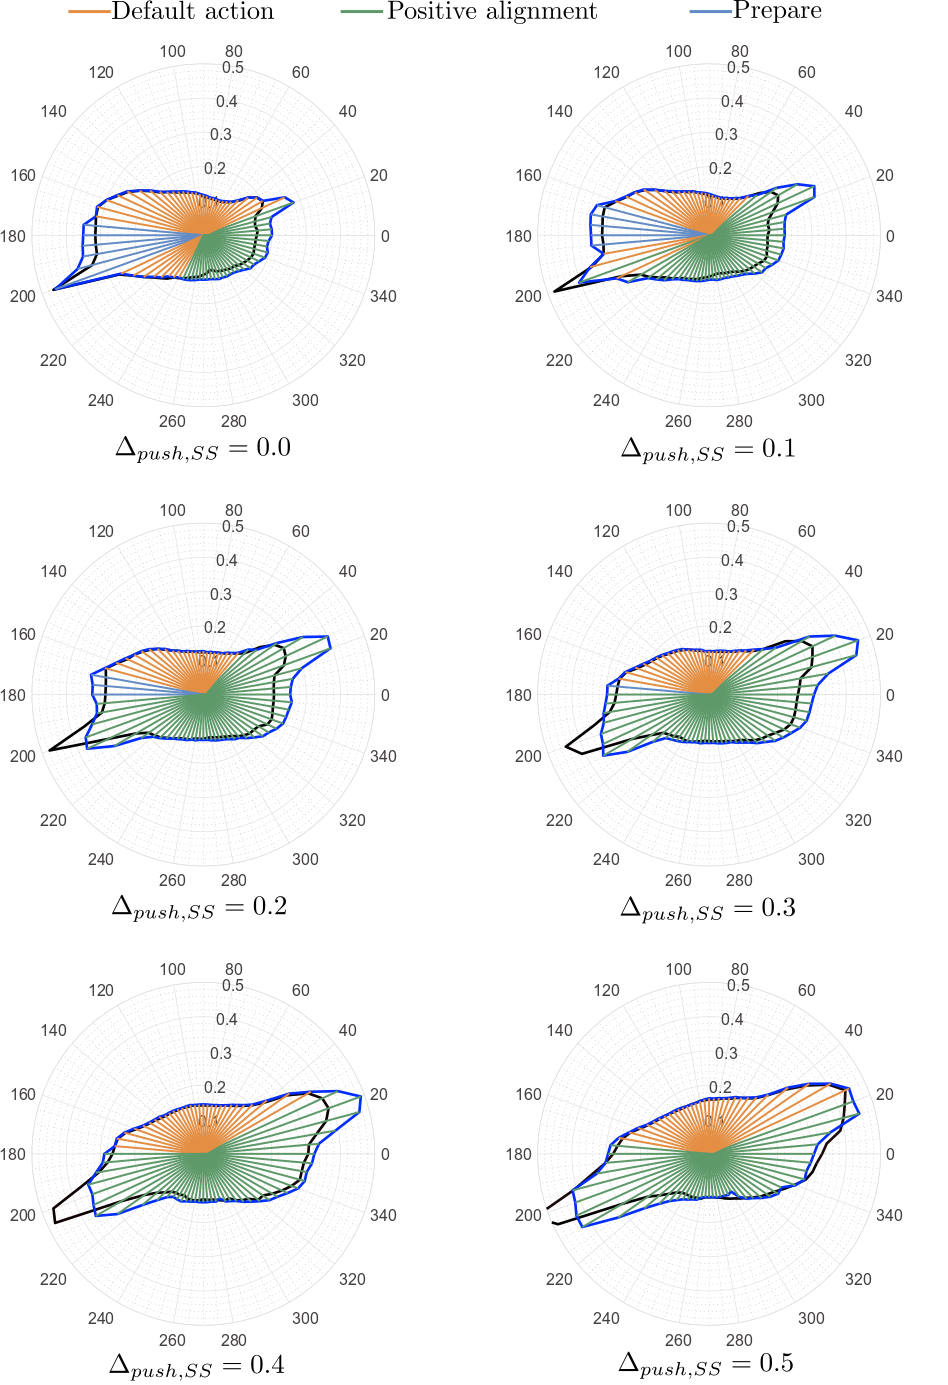
\includegraphics[width=0.85\textwidth]{STYLESTUFF/rounActions.png}
    \caption{Recoverable pushes for the default controller (black) and the vertical motion controller (blue). The radial lines show the actions used by the vertical motion control law.}
    \label{fig:roundPushActions}
\end{figure}

In \figref{fig:roundPushAng}, the maximum recoverable pushes are shown for when $\rcmpd$ is constrained to be inside the polygon, like in the previous figure, and when $\rcmpd$ is allowed to leave the polygon $5$ [cm]. Allowing $\rcmpd$ to go outside the polygon potentially requests angular momentum rate from the robot. However, this is highly dependent on the weights used in the whole-body \ac{QP}. Note how the plots with larger possible $\rcmpd$ locations seem to match shape with the plots where $\rcmpd$ is inside the polygon. Also note how for push directions coming from the back, the recovery is about the same for the default controller with larger $\rcmpd$ locations compared with the vertical motion controller where $\rcmpd$ is constrained to be inside the polygon.
\begin{figure}
     \centering
        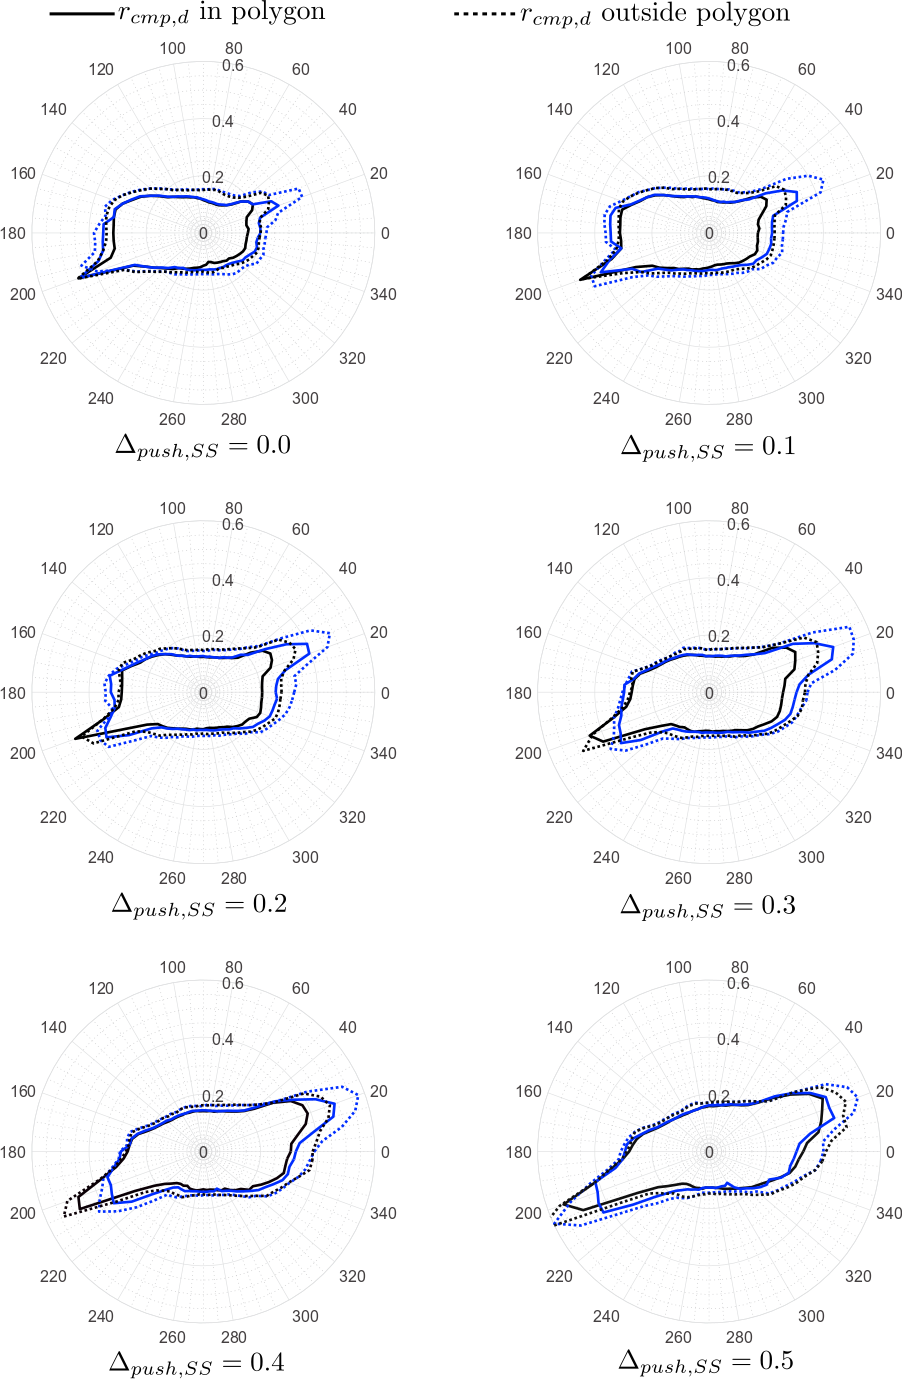
\includegraphics[width=0.85\textwidth]{STYLESTUFF/roundAng.png}
        \caption{Recoverable of the recoverable pushes for the default controller (black) and vertical motion controller (blue). A comparison is shown for when the desired \ac{CMP} is constrained to be inside the polygon, and when the desired \ac{CMP} is allowed to leave the polygon $0.05$ [m].}
        \label{fig:roundPushAng}
\end{figure}

\paragraph{A comparison of the response after equal impulses} is again conducted by applying the push where the default setup just recovered. A rear and frontal push are chosen to make a deeper evaluation of, which have a recoverable impulse of $i=0.156$ [m/s] and $0.315$ [m/s] respectively. In \figref{fig:walkplot}, time responses are shown for these applied impulses. For the vertical motion controller, the positive alignment action is used for the rear push and the prepare action is used for the frontal push, which can also be observed in \figref{fig:roundPushActions}. For the back push, the desired vertical linear momentum rate $\dotldz$ from a circle is clearly visible after the second `bang'. The maximum height violates the maximum allowed height for the controller slightly halfway swing. For the prepare action however, the minimum height stays above the minimum height constraint. From the reference and measured \ac{ICP} $\icpr$ and $\icp$ in the sagittal direction, it can be observed that the final \ac{ICP} error is smaller for the vertical motion controller.
\begin{figure}
     \centering
        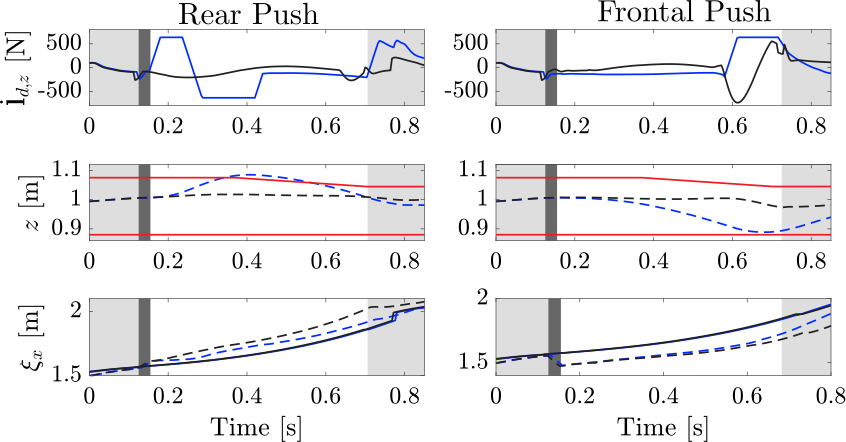
\includegraphics[width=0.99\textwidth]{STYLESTUFF/walkplot.png}
    \caption{Responses after a rear push of $i=0.156$ [m/s] and a frontal push of $0.315$ [m/s] is applied on Valkyrie for both control setups. The push is applied in the dark gray area and the light gray area shows where the robot is in \ac{DS}.}
    \label{fig:walkplot}
\end{figure}

\subsection{Atlas Hardware Results}
Additionally, some hardware tests on Atlas are conducted, triggering the positive alignment action. These tests are conducted on Atlas, as Atlas is able to walk faster than Valkyrie due to its more powerful actuation. Walking faster allows for \ac{CoM} positions at further distance from the \ac{CoP} positions, in which \ac{CoM} height variations have more effect on balance control. In \figref{fig:walk3D}, the walking pattern is shown that is used in the tests. Unlike in the Valkyrie simulations, a step length of $0.4$ [m] is used. The same \ac{SS} and \ac{DS} times as in the Valkyrie simulations could be used, which was about the maximum what the robot could do. Intermediate local pendulums between $\rcmpd$ and the \ac{CoM} are depicted after the push is applied with a constant time interval of $0.2$ [s]. The yellow lines show the projections on the $xz$-plane of the pendulums. The letters above the yellow lines match with letters below the images in \figref{fig:atw}; the pendulums are the $\rcmpd-\cxyz$ configurations for the images. At $a$ the push is applied and at $b$ released. The height change of the positive alignment action is clearly visible.
\begin{figure}
     \centering
        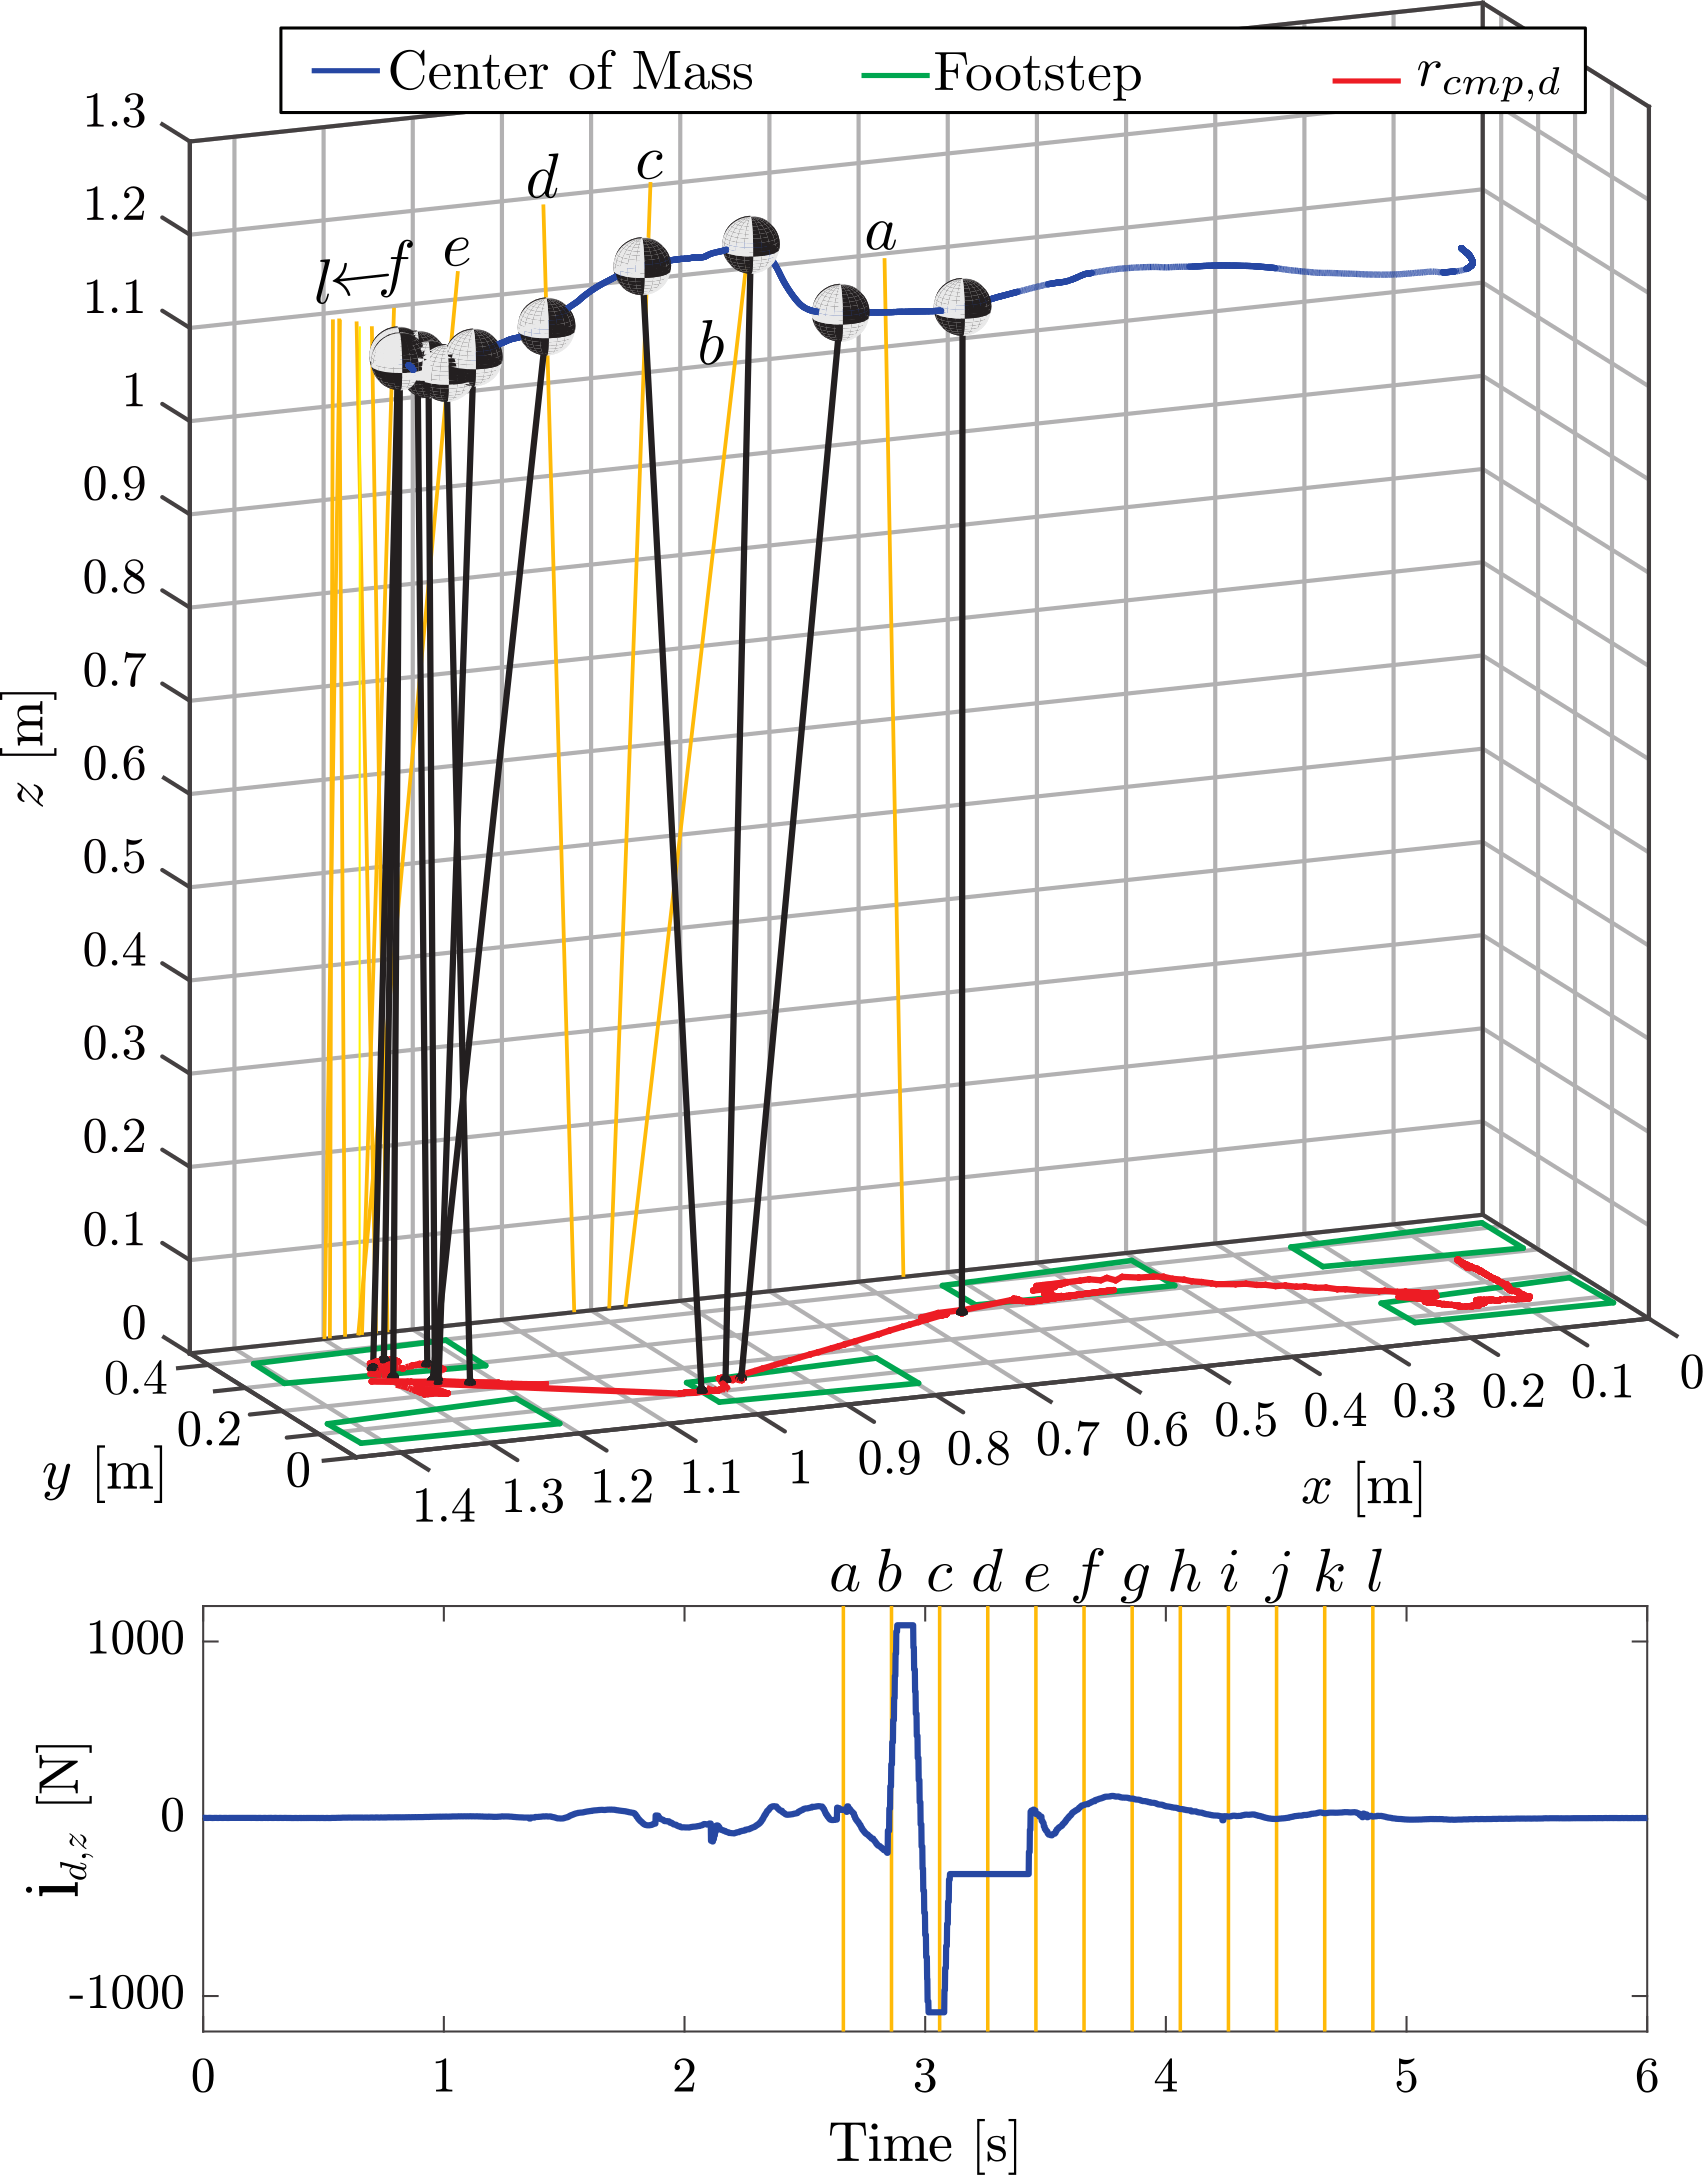
\includegraphics[width=0.99\textwidth]{STYLESTUFF/walk3D2.png}
        \caption{\ac{3D} plot of the \ac{CoM} and $\rcmpd$ trajectory during a walking push recovery test (top). The yellow lines are the pendulums projected on the $xz$-plane. The letters above the yellow lines correspond with the letters below the images in \figref{fig:atw} and show the $\rcmpd$-$\cxyz$ configurations. At $a$, the push is applied and at $b$ the push is released. Also, $\dotldz$ over time is shown (below).}
        \label{fig:walk3D}
\end{figure}

\begin{figure}
\centering
  \begin{tabular}{cccc}
    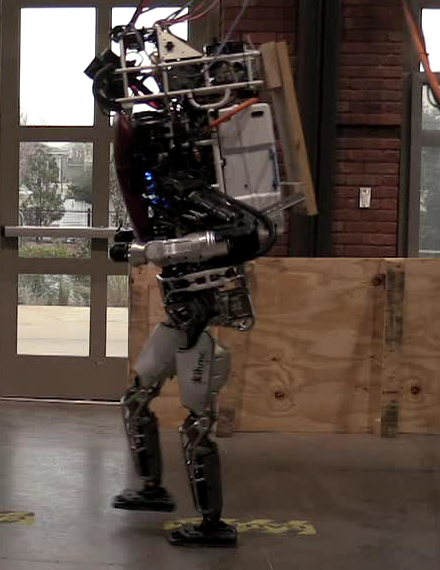
\includegraphics[width=1.4in]{STYLESTUFF/atw4} &
    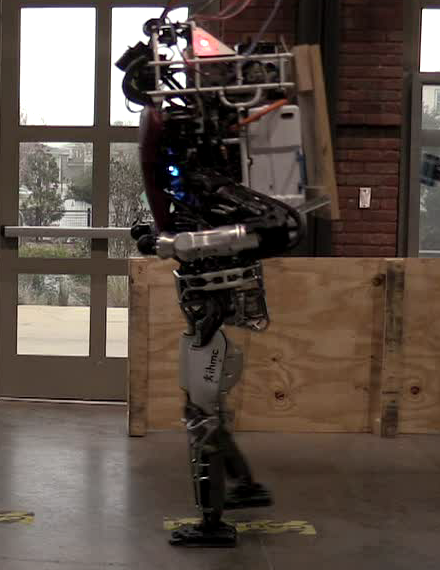
\includegraphics[width=1.4in]{STYLESTUFF/atw3} &
    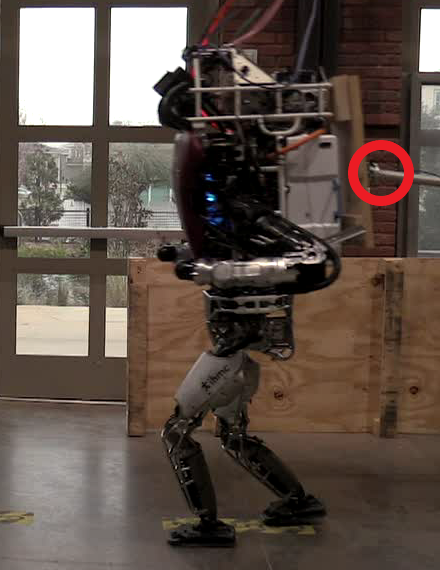
\includegraphics[width=1.4in]{STYLESTUFF/atw2p} &
    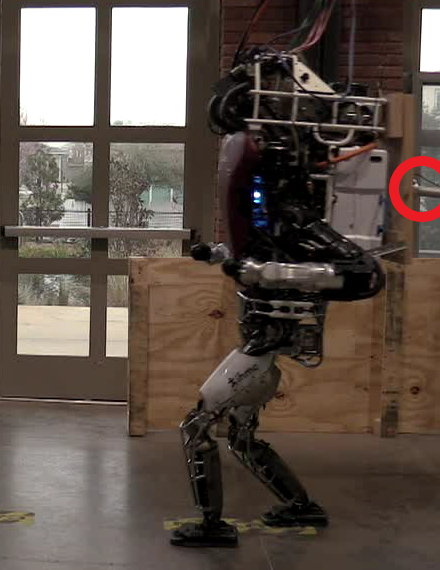
\includegraphics[width=1.4in]{STYLESTUFF/atw1p} \\
    $d$ & $c$ & $b$ & $a$ ~\\[2ex]
    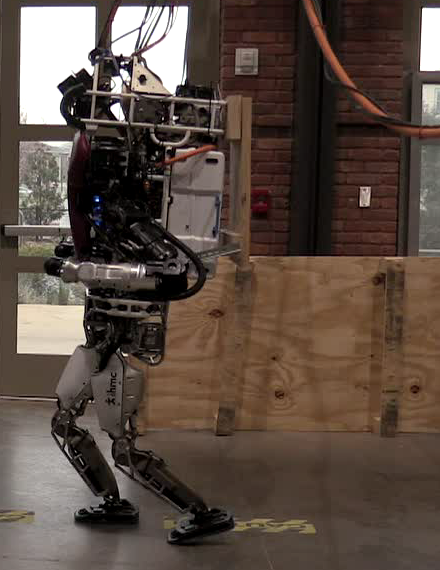
\includegraphics[width=1.4in]{STYLESTUFF/atw8} &
    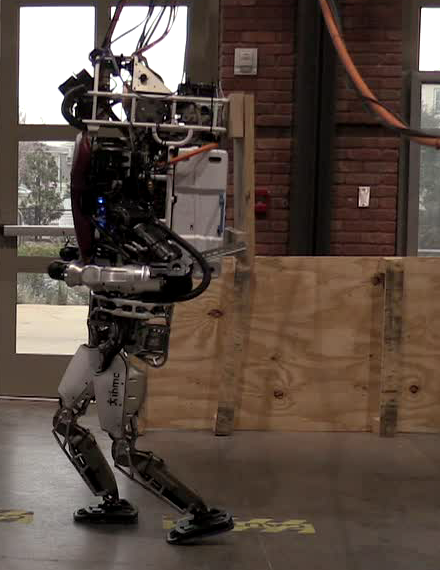
\includegraphics[width=1.4in]{STYLESTUFF/atw7} &
    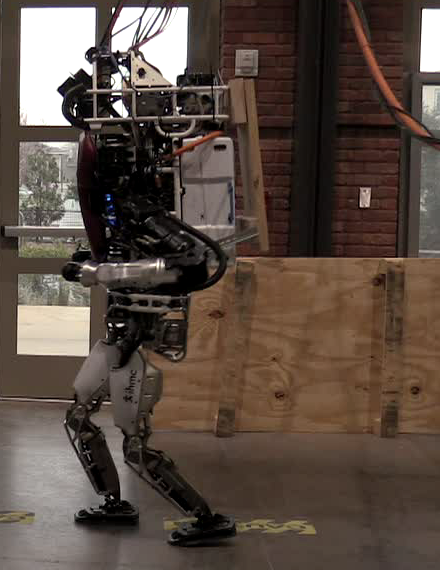
\includegraphics[width=1.4in]{STYLESTUFF/atw6} &
     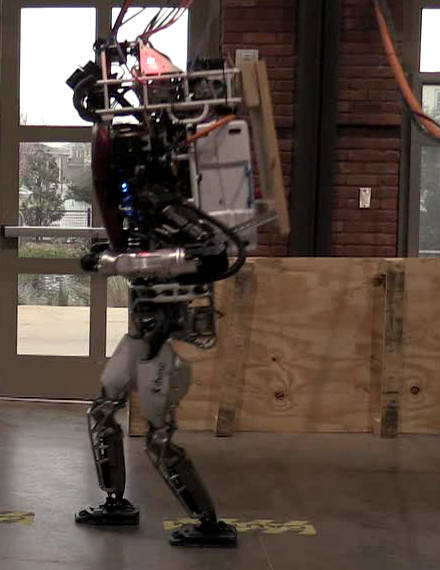
\includegraphics[width=1.4in]{STYLESTUFF/atw5} \\
     $h$ & $g$ & $f$ & $e$ ~\\[2ex]
    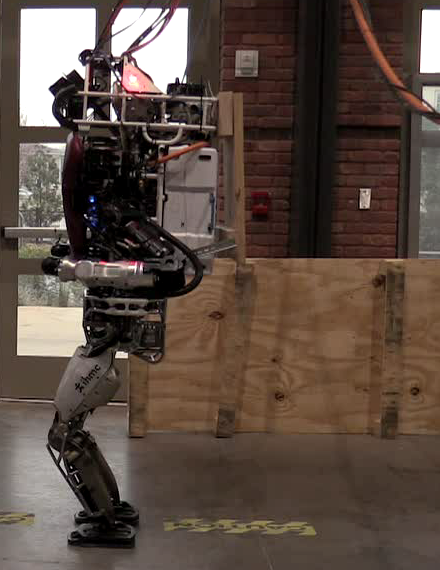
\includegraphics[width=1.4in]{STYLESTUFF/atw12} &
    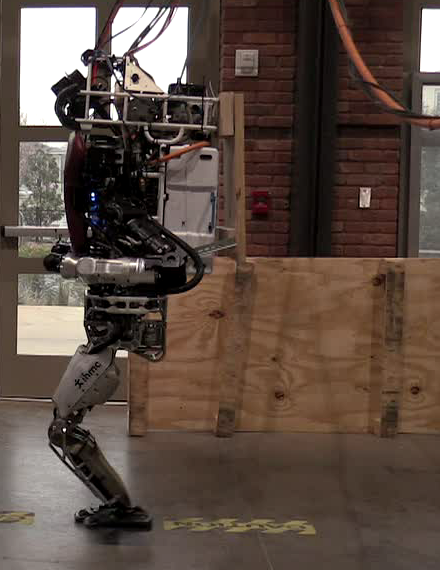
\includegraphics[width=1.4in]{STYLESTUFF/atw11} &
    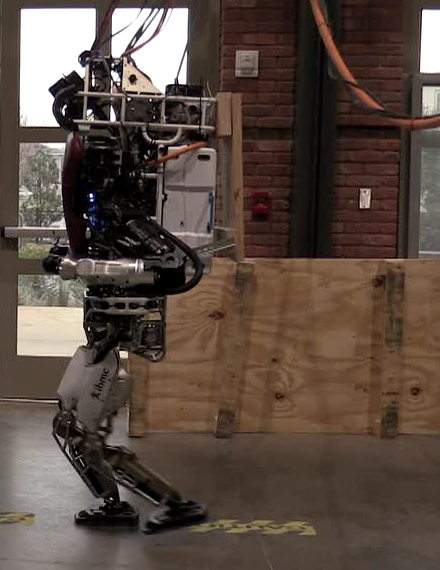
\includegraphics[width=1.4in]{STYLESTUFF/atw10} &
    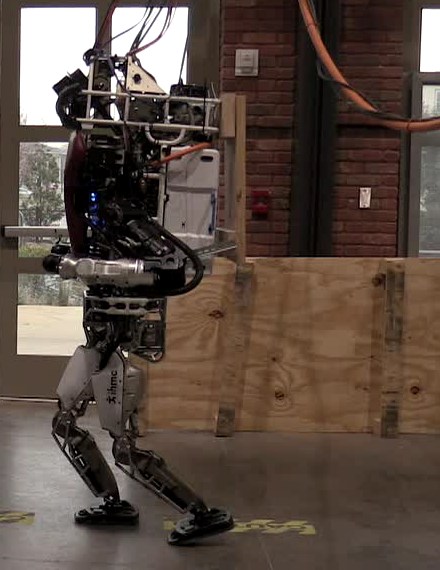
\includegraphics[width=1.4in]{STYLESTUFF/atw9} \\
    $l$ & $k$ & $j$ & $i$ 
  \end{tabular}
  \caption{Time-lapse of the positive alignment action on Atlas on hardware. The letters below the columns match with the corresponding letters above the yellow lines in \figref{fig:atw}. The push rod tip is encircled in red.}
  \label{fig:atw}
\end{figure}
% Discussion
\section{Discussion}
In this chapter, the control law of Chapter \ref{chap:standing} is extended for the use in \ac{3D}, using predefined strategies that can be heuristically be selected. These strategies rely on the predefined step time and location used in the control framework.

Like in the previous chapter, certain configurations are considered as `worst-case' scenarios. Again, a similar comparison with \ac{MPC} can be made. 

The relative distance $\delta$ and the alignment angle $\phi$ allow for making a heuristic decision for the use of height control in different configurations. Considering a bang-bang control law these variables could introduce, the control strategy relies on the proportional control of the rest of the framework. Any misalignment with the error would result in additional error when introducing the bang-bang action. This error can be controlled with future $\rcmpd$ positions.

From the results obtained for the step time and length considered, it seemed that height control in the beginning of \ac{SS} results in the most improvement compared to strategies that do not use \ac{CoM} height variation. The vertical motion controller performs worse than the default setup around the $200$ degree push direction for all push moments in swing $\fracpush$ considered. This may be a results of the chosen control actions based on the thresholds $\phimin$, $\phimax$ and $\deltamin$.

Also a comparison is made for cases where $\rcmpd$ could leave the polygon. For the use of additional height variation, the $\rcmpd$ would be projected on the polygon to get a $\rcopd$, with the motivation that no additional angular momentum rate would be needed to achieve the commanded desired linear momentum rate on the robot. When the \ac{CMP} is outside the polygon, the robot uses torque about the \ac{CoM}, as can be derived from Section \ref{sec:grp}. However, only desired linear momentum rate is commanded in the framework based on $\rcmpd$, which results in the use of angular momentum rate by the robot to be highly depending on the weights chosen for the objectives in the \ac{QP}. The weights used for these tests are the default weights used on Valkyrie, see Appendix \ref{chap:params}.
